\documentclass{article}
%documentclass[draft]{article}

\usepackage[italian]{babel}
\usepackage[utf8]{inputenc}


\usepackage{graphicx} % Immagini fantastiche e...
\graphicspath{        % dove trovarle
  {./images/},
  %{../images/}        % Necessario se cartella chapters
}

%% Bibliografia
\usepackage{csquotes}
\usepackage{biblatex}
\addbibresource{bibl.bib}


% Grafici direttamente in latex
\usepackage{tikz}
\usetikzlibrary{shapes,positioning,calc}
\colorlet{lightgray}{gray!20}

\usepackage{rotating} % per tabella ruotata
\usepackage{makecell}
%\usepackage[showframe=true]{geometry}
\usepackage{changepage}

% Immagini galleggiano
\usepackage{float}

\usepackage{color}

\usepackage{caption}
% per caption ad immagini in tab annidiate
\usepackage{subcaption}

\usepackage{hyperref} % lasciare per ultimo
%\hypersetup{colorlinks=true, linkcolor=blue, citecolor=black, plainpages=false, urlcolor=blue}
\hypersetup{colorlinks=true, linkcolor=black, citecolor=black, plainpages=false, urlcolor=blue}

% Usato nella copertina
\usepackage{wallpaper}



% Per blocchi di codice
%\usepackage{listings}
% Esempio di impostazione per listings
%\stset{
%   language=Octave,
%   % language=Matlab,
%   showspaces=false,
%   showstringspaces=false,
%   basicstyle=\ttfamily,
%   %numbers=left,
%   numbers=none,
%   numberstyle=\small,
%   mathescape,
%}
%\newcommand*\lstinputpath[1]{\lstset{inputpath=#1}}
%\lstset{ % per apici e pedici nel codice
%  mathescape,
%  numbers=none
%}
%\lstset{ numbers=none }

%\usepackage{listings}
%
%\definecolor{darkblue}{rgb}{0,0,.75}
%%\lstloadlanguages{Matlab} %use listings with Matlab for Pseudocode
%\lstnewenvironment{PseudoCode}[1][] {
%  \lstset{
%    mathescape=true,
%    %language=Matlab,
%    basicstyle=\scriptsize,
%    keywordstyle=\color{darkblue},
%    numbers=left ,
%    xleftmargin=.04\textwidth,
%    %#1
%  }
%}
%{}

\usepackage{algpseudocode,algorithm,algorithmicx}
%\newcommand*\DNA{\textsc{dna}}
%
%\newcommand*\Let[2]{\State #1 $\gets$ #2}
%\algrenewcommand\algorithmicrequire{\textbf{Precondition:}}
%\algrenewcommand\algorithmicensure{\textbf{Postcondition:}}






% Simboli matematici
%\usepackage{amsthm}
\usepackage{amssymb}
\usepackage{amsmath}
%\usepackage{amsfonts}
%\usepackage{mathabx} % per \topdoteq
%\usepackage{mathtools, amsthm}


% Comodo per evidenziare zone da modificare
\usepackage{todonotes} 

% Lorem ipsum...
\usepackage{lipsum} 


 
% ================================ %
%          Cose Personali          %
% ================================ %

% Alcune comodita' logico/matematiche
\let\ep\epsilon
\let\b\bullet
\let\iff\Leftrightarrow
\newcommand{\viff}{\Updownarrow}
\let\impl\Rightarrow

\newcommand{\norm}[1]{\lvert\lvert #1 \lvert\lvert}
\newcommand{\Norm}[1]{\Big\lvert \Big\lvert #1 \Big\lvert \Big\lvert}

\newcommand\N{\ensuremath{\mathbb{N}}}
\newcommand\R{\ensuremath{\mathbb{R}}}
\newcommand\Z{\ensuremath{\mathbb{Z}}}
\renewcommand\O{\ensuremath{\emptyset}}
\newcommand\Q{\ensuremath{\mathbb{Q}}}
\newcommand\C{\ensuremath{\mathbb{C}}}

\newcommand\E{\ensuremath{\mathbb{E}}}
\newcommand\T{\ensuremath{\mathbb{T}}}
\renewcommand\inf{\ensuremath{\infty}}




% ================================ %
%            Il Documento          %
% ================================ %
\begin{document}

% ================================ %
%        Creo Prima Pagina         %
% ================================ %

\ThisCenterWallPaper{0.95}{polloPallido}
% Intestazione
% TODO Migliorare esteticamente
\begin{titlepage}
 	\centering
  \Huge{\textbf{Approfondimento di Intelligenza Artificiale}}\\
 	[30mm]
 	\centering
  \Huge{\textbf{Studente: Tristano Munini}}\\
 	%[25mm]
  %\raggedright
  %\Large{\textbf{Corso:}}\\
  %\Large{\textbf{TODO}}\\
 	[125mm]
 	\centering
  \LARGE{\underline{\textbf{ANNO ACCADEMICO 2019-2020}}}\\
\end{titlepage}

%% ================================ %
%%              Indice              %
%% ================================ %
%\tableofcontents
%\thispagestyle{empty}
%\cleardoublepage
%\setcounter{page}{1}


% ================================ %
%      Qua Inizia La Tesina        %
% ================================ %
%\abstract{
%  \lipsum[1]
%}

%\pagenumbering{gobble} % TODO REMOVE

%\input{./chapters/x.tex}
%%!TEX TS-program = pdflatex
%!TEX root = main.tex
%!TEX encoding = UTF-8 Unicode

\section{Introduzione}

Questo approfondimento ha come oggetto le tecniche di \emph{Machine Learning} (ML) \emph{Generative Adversarial Network} (GAN) e \emph{Reinforcement Learning} (RL).
In  particolare nelle  prima sezione si  esplorano le tecniche generative, definendo prima i \emph{Variational  Autoencoder} e  poi le GAN.
Nella seconda sezione si definiscono i concetti alla base  del  \emph{Reinforcement Learning} e come le tecniche di ML possono essere sfruttate in questo ambito.
La terza  sezione illustra come si può combinare l'architettura GAN con tecniche prese dal mondo del RL per generare testi sintetici che siano verosimili.
Nello specifico si analizzano l'architettura SeqGAN \cite{SeqGAN} e la sua evoluzione LeakGAN \cite{LeakGAN}.
L'ultima sezione illustra brevemente un'implementazione delle LeakGAN scritta dagli stessi autori dell'articolo che la introduce \cite{LeakGAN}.

%%!TEX TS-program = pdflatex
%!TEX root = main.tex
%!TEX encoding = UTF-8 Unicode


\section{GAN}
Uno tra i primi metodi che permettevano di generare immagini sintetiche faceva uso di una particolare versione di \emph{Auto-Encoder} i \emph{Variational Auto-Encoder}.
Come nel caso degli AE classici, i VAE hanno una struttura che ricorda una clessidra: la prima metà della rete permette di comprimere l'input, mappandolo in quello che viene chiamato spazio latente, di minor dimensione rispetto allo spazio di partenza;  la seconda metà, invece, prende l'input compresso e lo mappa nello spazio di partenza.
Durante il training si vuole ottimizzare la compressione in modo che non ci sia perdita di informazione, questo viene effettuato andando a minimizzare la distanza tra input originale ed input ricostruito.
Nei VAE, in corrispondenza del punto della rete in cui si raggiunge il livello massimo di compressione (\emph{bottleneck}), invece di essere generato il vettore compresso $z$, viene prodotta una coppia di vettori $\sigma$ e $\mu$ che descrivono una distribuzione di probabilità dei vettori compressi.
In questo modo è possibile campionare $z$ dalla distribuzione appena prima della decompressione.
Il campionamento non è un'operazione differenziabile e questo rende inapplicabile l'algoritmo della $backpropagation$, quindi risulta necessario effettuare quello che viene chiamato \emph{reparametrization trick}.
Rappresentando $z$ come $z = \mu + \sigma \odot \varepsilon$ in cui $\varepsilon \sim \mathcal{N}(0,1)$, quindi $\varepsilon$ è campionata da una distribuzione normale, è possible effettuare l'operazione di \emph{sampling} all'esterno della rete.
In questo modo $\mu$ e $\sigma$ possono essere utilizzati per il calcolo del gradiente e quindi usati durante la \emph{backpropagation}.

Dopo questa breve panoramica sulle VAE, ispirata alla lezione del MIT \cite{MIT_GEN}, ci si accorge che sono una soluzione astuta ma complessa e che le loro prestazioni sono vincolate strettamente allo spazio latente che si è trovato durante il training.
%TODO nota sul Disentanglement delle variabili che permette di avere controllo sulle singole caratteristiche delle immagini generate

Le \emph{Generative Adversarial Network} (GAN) sono state modellate appositamente per trovare un'altra soluzione al problema della creazione di immagini sintetiche.
Nelle GAN sono presenti due modelli che, citando \cite{GANTF}, \emph{``vengono addestrati simultaneamente da un processo contraddittorio. Un generatore ("l'artista") impara a creare immagini che sembrano reali, mentre un discriminatore ("il critico d'arte") impara a distinguere le immagini reali dai falsi''}.
Riformulando la frase si può dire che una GAN, come si vede in \autoref{fig:gan}, è composta da due reti: la prima viene chiamata Generatore $G$ ed il suo scopo è fornire in output un $x_{fake}$ che sembri appartenere alla distribuzione del \emph{dataset} reale fornito; la seconda, detta Discriminatore $D$, prende in input un $x_{fake}$ ed un $x_{real}$ estratto dal \emph{dataset} e deve riuscire a distinguere il dato reale da quello sintetico.
Quindi il training viene svolto in quattro momenti:
\begin{itemize}
  \item all'inizio $G$ a partire da del rumore randomizzo genera, basandosi sulle sue conoscenze attuali, un $x_{fake}$;
  \item successivamente $D$ stabilisce quale tra $x_fake$ ed un $x_real$ fornito è sintetico;
  \item la prestazione di $D$ viene valutata con il \emph{ground truth} e con questa può essere effettuata la \emph{backpropagation} su $D$;
  \item con l'output del discriminatore è possibile determinare anche la prestazione di $G$, infatti se questo è riuscito a confondere $D$ significa che sta raggiungendo una buona conoscenza del dominio.
\end{itemize}
Notare come $G$ sia in grado di mappare del rumore casuale nello spazio delle \emph{feature} del dominio e che quindi, una volta allenato, possa essere sfruttato molto facilmente: basterà avere del rumore da cui partire.
Si può quindi dire che $G$ opera come il decoder di un AE con un particolare spazio latente molto semplice.
\begin{figure}[ht]
  \centering
  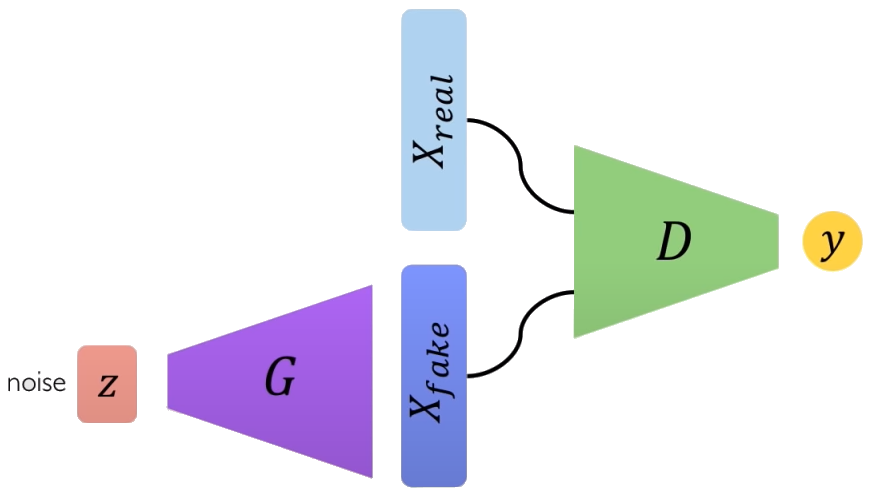
\includegraphics[width=.7\textwidth]{GAN/arch.png}
  \caption{Architettura di una generica GAN (dalle slide in \cite{MIT_GEN})}
  \label{fig:gan}
\end{figure}
Rispetto ai $VAE$ le $GAN$ risultano non solo più intuitive ma permettono anche di raggiungere prestazioni veramente sorprendenti, come si può vedere in \cite{GAN_HD}, in cui anche gli esperti umani vengono ingannati dai prodotti della rete.

Va fatto notare però che le GAN sono notoriamente difficili da allenare %\cite{HARD_GAN}
\todo{leggere xke GAN difficili}
, basti pensare che prima dell'allenamento entrambe le sotto-reti non hanno alcuna conoscenza del dominio e si chiede loro di guidarsi a vicenda.
Se il discriminatore converge rapidamente è possibile che dia una valutazione così bassa al generatore da causare il \emph{vanishing gradient problem}, rendendo quindi impossibile che $G$ possa migliorarsi.
Un altro problema noto è quello del \emph{model collapse} che si verifica quando $G$ riproduce molto bene soltanto una piccola frazione del dominio.
In questo modo riesce ad ottenere punteggi molto alti ma a discapito della generalità.


% L'efficacia di questa tecnica e' lampante quando si parla di immagini...
%In questo caso si fa riferimento alla possibilità di utilizzare le GAN come generatori di immagini sintetiche indistinguibili da quelle reali, in \cite{GAN_HD} si può osservare il livello di dettaglio impressionante che queste reti sono in grado di produrre.


\todo[inline]{aggiungere robe dal paper originale se si deve allungare}

$$
min_G max_D V(D,G) = \E_{x \sim P_real(x)} [ log D(x) ] 
+
\E_{z \sim P_z(x)} [ log ( 1 - D(G(x)) ]
$$ 
\todo{inserire formula per chiarire training e obj}

%\clearpage
%%!TEX TS-program = pdflatex
%!TEX root = main.tex
%!TEX encoding = UTF-8 Unicode


\section{RL}
Il \emph{Reinforcement Learning} (RL), assieme al \emph{Supervised Learning} ed all'\emph{Unsupervised Learning}, è il terzo paradigma di apprendimento autonomo.
Gli ultimi due paradigmi sfruttano un dataset, rispettivamente con e senza label, per portare a termine un specifico task oppure generare nuova informazione.
Nel caso del RL il dataset viene sostituito con un ambiente (\emph{environment}) nel quale il modello può eseguire delle azioni e osservarne le conseguenze, quindi come l'ambiente viene modificato dall'azione appena compiuta.
In questo paradigma il modello viene anche chiamato ``agente'' e l'elenco, discreto oppure continuo, delle azioni eseguibili prende il nome di \emph{action space}.
L'agente impara grazie ad una ricompensa (\emph{reward}), positiva o negativa, associata al risultato delle sue azioni.
Il suo obiettivo è quello di massimizzare la somma dei \emph{reward} sul lungo termine, quindi si vuole che scopra e adotti una strategia (\emph{policy}) efficace nell'ambiente considerato.
Poiché è necessario svolgere numerose iterazioni del tipo \emph{trial-and-error} e considerato che solitamente un fallimento corrisponde anche ad una grande acquisizione di informazione, bisogna creare degli \emph{environment} virtuali che siano il più vicino possibile al dominio di applicazione finale e che permettano un'esecuzione rapida e senza costi aggiuntivi.
%
%\todo{ampliare intro?} % TODO
%\todo{esempi con ref?} % TODO

Riprendendo quanto illustrato in \cite{MIT_RL} ed in \cite{Simple_RL}, una prima modellazione sfrutta una funzione che valuta la qualità dell'azione svolta 
$$
Q(s_t, a_t) = \E [ R_t | s_t, a_t]
$$
in cui 
$s_t$ è lo stato corrente cioè come l'ambiente si presenta all'agente,
$a_t$ è l'azione che l'agente svolge all'istante $t$,
mentre a destra dell'uguale si ha il valore atteso del \emph{reward} totale $R_t$ che l'agente potrà ricevere in futuro, quindi negli $s_{t+i}$ con $i=1,2,\dots$ se esegue $a_t$ in $s_t$.
Calcolare $R_t$ risulta critico perché la sua naturale definizione è
$$
R_t = \sum_{i=t}^{\inf} \gamma^i r_i = 
\gamma^{t+1} r_{t+1} + 
\gamma^{t+2} r_{t+2} + 
\gamma^{t+3} r_{t+3} + \dots
\gamma^{t+n} r_{t+n} + \dots
$$
in cui $0 < \gamma < 1$  viene chiamato \emph{discount factor} ed indica la \emph{greediness} del modello. %\todo{spiegare meglio in caso}
In questa casistica risulta utile approssimare $Q(s,a)$ con una rete neurale, in questo modo si evita di dover fissare a mano un \emph{hyperparameter} come, ad esempio,  il numero di somme da effettuare per approssimare $R_t$.
L'idea è fornire alla rete, detta anche \emph{Q-Network} \cite{DQN}, lo stato corrente ed ogni possibile azione lecita e successivamente scegliere l'azione a cui la rete assegna il valore più alto.
$$
argmax_a Q(s_t, a) %\quad\textrm{con $Q(\cdot)$ approssimata da una rete}
$$
Procedendo in questo modo per ogni stato che si incontra $s_{t+i}$ con $i=1,2,\dots$ è possibile seguire una policy $\pi(s)$ ottimale ad ogni passo.
La policy $\pi(s)$ è una politica di scelta che associa uno stato ad un'azione, con lo scopo di ottenere un buon guadagno sul lungo termine.
Si trova una strategia ottimale quando ogni scelta fatta seguendo la $\pi$ è ottimale.

\todo[inline]{qui mettere loss function e spiegarla?}

L'approccio appena presentato richiede che l'\emph{action space} sia discreto e di dimensione ridotta, altrimenti sarebbe impossibile o molto costoso iterare su tutte le azioni per selezionarne la migliore.
Per ovviare a questo problema si possono utilizzare modelli che provano ad ottimizzare direttamente la \emph{policy} $\pi(s)$, questi modelli prendono il nome di \emph{Policy Learning} e vengono allenati tramite il \emph{Policy Gradient}. %\todo{cite paper?}
In questo modo è possibile ottenere direttamente l'azione migliore a partire soltanto dallo stato.
L'idea principale è approssimare $\pi$ con una distribuzione di probabilità, in questo modo risulta naturale utilizzare un \emph{action space} continuo, inoltre si può ottenere una strategia non deterministica, quindi più flessibile e con maggiori capacità esplorative durante il training.
Il non determinismo è introdotto quando, per scegliere l'azione da eseguire, se ne estrae una dalla distribuzione di probabilità data dalla \emph{policy}.
In formule, dato uno stato $s$ l'azione $a$ verrà estratta secondo:
%$$
%a = 
%\pi(s) \sim P(a|s) \quad\textrm{in cui } \sum_{a_i \in A} P(a_i | s) = 1 \quad\textrm{con $A$ \emph{action space}}
%$$
$$
a = 
\pi(s) \sim P(a|s) \quad\textrm{in cui } \int_{a = - \inf}^{\inf} P(a | s) = 1
$$
Poiché $P(a|s)  = \mathcal{N}(\mu,\sigma ^2)$ si può fare in modo che la rete dia in output direttamente il vettore della medie $\mu$ e il vettore delle varianze $\sigma^2$.
L'allenamento incomincia con l'inizializzazione dell'agente e dell'ambiente, poi l'agente segue la sua policy corrente fino a terminazione mentre tutti gli stati, le azioni e i reward vengono registrati.
Infine si aumenta la probabilità delle azioni che hanno portato a reward positivi e si decrementa la probabilità delle azioni con reward negativo, fatto ciò si effettua nuovamente l'inizializzazione in modo da valutare la policy aggiornata. 
Notare che definire il concetto di ``terminazione'' non è sempre ovvio e può corrispondere, ad esempio, all'esecuzione di un numero limitato di azioni oppure al ricevimento di un grande reward negativo.
L'aggiornamento dei pesi della rete, quindi della policy, viene effettuato tramite \emph{gradient descent} usando la \emph{loss}
$$
loss = - log P(a_t | s_t ) R_t
$$
Il logaritmo indica la probabilità logaritmica con cui $a_t$ viene scelta allo stato $s_t$ mentre $R_t$ è il valore atteso del reward totale che si guadagnerà.
Se $R_t$ è positivo allora converrà aumentare la probabilità di selezionare $a_t$, viceversa se è negativo conviene diminuire la probabilità.
Il \emph{Policy Gradient} è il gradiente relativo a questa particolare \emph{loss}.

\todo[inline]{TODO più matematicoso con spiegazione calcolo $R_t$}
\todo[inline]{TODO introdurre REINFORCE?}
\todo[inline]{TODO differenza tra esplorare e exploit}
\todo[inline]{TODO esempio Alpha GO, Alpha Zero e Hide and Seek}

\clearpage


\todo[inline]{quattro parole sulle LSTM}
%\clearpage
%!TEX TS-program = pdflatex
%!TEX root = main.tex
%!TEX encoding = UTF-8 Unicode


\section{GAN+RL per testi}
In questa sezione vengono illustrati due modelli capaci di generare testi sintetici sfruttando un'architettura GAN in cui $G$ viene allenato attraverso \emph{Reinforcement Learning}.
Il primo modello, chiamato SeqGAN, è stato presentato in \cite{SeqGAN} ed illustrato anche in \cite{GAN_for_text}; il secondo è evoluzione del primo, permette di generare testi più lunghi, prende il nome di LeakGAN ed è descritto in \cite{LeakGAN}.
Si vuole anche citare \cite{NetTextGen_Review} in cui vengono illustrati alcuni modelli usati prima delle SeqGAN e quelli sviluppati successivamente fino ad arrivare alle LeakGAN.
Nell'articolo si trova anche un confronto tra MaliGAN, RankGAN, MaskGAN e TextGAN, non trattate in questo documento.
%\todo[inline]{Sono particolarmente interessanti perché con SeqGAN si risolve} % TODO se serve

\subsection{SeqGAN}
Come riportato nell'introduzione dell'articolo \cite{SeqGAN}, per generare frasi che siano verosimili è necessario allenare un discriminatore che valuti frasi intere e che assegni a queste un punteggio.
Purtroppo ciò rende molto difficile allenare il generatore, perché non è possible determinare se un punteggio basso corrisponde all'intera struttura della frase oppure soltanto ad una o poche parole.
La problematica è ancora più evidente nel caso in cui il generatore è una RNN% \todo{mai introdotte per ora, TODO da fare mini sezione sopra?}
rendendo difficile, ad esempio aggiornare efficacemente il modo con cui vengono create le parti iniziali di frasi.

Le SeqGAN affrontano il problema in un modo molto interessante: se si considera il punteggio che $D$ fornisce alle frasi come \emph{reward} per $G$ e se questo utilizza come stato la frase generata fino ad ora e come azione la scelta della parola successiva, allora è possibile sfruttare il \emph{Policy Gradient} sul generatore.
Di fondamentale importanza la \emph{Monte Carlo Search} con \emph{Rollout} che viene effettuata per valutare la bontà di frasi incomplete, così da alterare efficacemente la distribuzione della parola che ancora deve essere scelta: 
durante la generazione di una frase, $G$ non può ricevere una valutazione da $D$ perché il discriminatore è in grado di valutare soltanto frasi intere % TODO fare osservazione? % (una frase incompleta sarà sempre poco verosimile 
quindi vengono generate $N$ frasi con prefisso la frase generata fino ad ora.
Si sfrutta poi $D$ per valutare tutte le $N$ frasi e si effettua una media dei \emph{reward} ottenuti, così si ottiene il valore atteso della bontà della frase che si sta generando.
Ci si riferisce a questo furbo accorgimento come \emph{N-Monte Carlo Search} con \emph{Rollout}.

Riprendendo i formalismi usati nell'articolo si ha:
\begin{itemize}
  \item un modello generativo $G_\theta$, con $\theta$ si indica i parametri interni, in grado di generare sequenze $Y_{1:T} = ( y_1, \dots , y_t, \dots , y_T)$ con gli $y_t$ appartenenti all'insieme dei token validi $\T$;
  \item al tempo $t$ lo stato $s$ equivale ai token prodotti fino ad ora $(y_1, \dots , y_{t-1})$ mentre l'azione $a$ è il prossimo token da selezionare $y_t$;
  \item con $G_\theta (y_t | Y_{1 : t-1} )$ si indica il modello non deterministico descritto.

  \item Il modello discriminativo $D_\phi$, con parametri $\phi$, è in grado di fornire la probabilità $D_\phi ( Y_{1:T})$ che $Y_{1:T}$ sia stato estratto dai dati reali.
\end{itemize}
% TODO \todo[inline]{qui immagine rete?}

Prima di continuare con la \emph{loss function} e la formulazione della \emph{Monte Carlo Search}, 
va sottolineato che il modello RNN è leggermente diverso da quello classico, infatti ad ogni passo la rete prende in input il token generato al passo precedente anziché riceverlo dall'esterno.
Si può quindi dire che assomigli ai modelli RNN usati come decoder durante la traduzione di testi, nei quali lo stato interno e l'ultima parola tradotta vengono utilizzati per aggiornare lo stato e generare la parola successiva.
%\todo{add ref to \url{https://arxiv.org/pdf/1506.03099v1.pdf}}
%Notare anche che la codifica interna 
%Si fa presente che lo stato di partenza è TODO e l'input è parte da \todo[inline]{partenza con $s_0$ come viene fatta? $h_0$ com'è?}
%Si può notare come questa sia la rivisitazione del tipico input randomico $z$ di una generica GAN.
Il primo token, o stato di partenza, è un token particolare che si indica con $s_0$.
Lo stato $h_0$ di partenza può essere fissato oppure selezionato casualmente così da da modificare il punto di partenza (simili all'input $z$ per i VAE).
L'obiettivo del generatore $ G_\theta $ è quello di produrre una sequenza a partire dallo stato $s_0$ che massimizzi il \emph{reward} totale, in formule:
$$
J(\theta) = \E[R_t | s_0, \theta ] =
\sum_{y_1 \in \T}
G_\theta ( y_1 | s_0) \cdot
Q_{D_\phi}^{G_\theta} ( s_0, y_1)
$$
in cui $Q_{D_\phi}^{G_\theta} ( s, a)$ è la funzione che indica il \emph{reward} accumulabile eseguendo l'azione $a$ allo stato $s$ e seguendo la \emph{policy} $G_\theta$ nei passi successivi.
Questa funzione dovrà necessariamente essere stimata, perché sappiamo che $D_\phi$ non può essere sfruttato su sequenze incomplete.
Quindi si utilizza una \emph{$N$-Monte Carlo Search} con \emph{Rollout} per stimare $N$ volte i $T-t$ token mancanti
$$
\{ 
  Y_{1:T}^1,
  \dots,
  Y_{1:T}^N
\}
=
MC (Y_{1:t}; N)
$$
Gli $ Y_{t+1:T}^n $ con cui si completa la sequenza parziale sono campionati usando la stessa \emph{policy} $G_\theta$.
Quindi la stima del \emph{reward} atteso è data da
%$$
%Q_{D_\phi}^{G_\theta} ( s_0, y_1) TODO
%=
%\left\{
%\begin{array}{lr}
%  x(n), & \text{for } 0\leq n\leq 1\\
%\end{array}
%\right\
%$$

$$
Q_{D_\phi}^{G_\theta}
( s = Y_{1:t-1} ,
a = y_t)
=
\left\{\begin{array}{lr}
    \dfrac{1}{N} \sum_{n=1}^N D_\phi (Y_{1:T}^n) ,\; Y_{1:T}^n \in MC(Y_{1:t};N)
      & \textrm{for } t < T \\

    D_\phi (Y_{1:t}) & \textrm{for } t = T

\end{array}\right.
$$
%Abbiamo visto come $J(\theta)$ può essere calcolata e sappiamo che 

Per quanto riguarda il discriminatore $D_\phi$ viene specificato che l'aggiornamento dei suoi parametri $\phi$ viene effettuato solo quando il generatore ha creato un numero sufficiente di sequenze.
In questo modo è possibile avere un discriminatore che si adatta e migliora assieme al generatore, pur lasciandogli il tempo di perfezionarsi.
In formule $D_\phi$ viene allenato secondo:
$$
min_\phi
- \E_{Y \sim p_{real}} [ log D_\phi (Y) ]
- \E_{Y \sim G_\theta} [ log ( 1 - D_\phi(Y))]
$$
L'algoritmo del train illustrato in \cite{SeqGAN} è riportato in \textbf{Algorithm \ref{alg:SeqGAN}}.
\begin{algorithm}
  \caption{Sequence Generative Adversarial Nets}
  \label{alg:SeqGAN}
  \begin{algorithmic}[1]
    \State Initialize $G_\theta$, $D_\phi$ with random weights $\theta$, $\phi$
    \State Pre-train $G_\theta$ using MLE on real data
    \State Generate negative samples using $G_\theta$ for training $D_\phi$
    \State Pre-train $D_\phi$ via minimizing the cross entropy
    \Repeat
      \For{g-steps}
        \State Generate a sequence $Y_{1:T} = (y_1, \dots , y_T) \sim G_\theta$
          \For{$t$ in $1:T$}
            \State Compute $Q_{D_\phi}^{G_\theta}(s=Y_{1:T}; a=y_t)$
          \EndFor 
        \State Update generator parameters via policy gradient
      \EndFor 
      \For{d-steps}
        \State Use current $G_\theta$ to generate negative examples and combine with given positive examples
        \State Train $D_\phi$ for $k$ epochs
      \EndFor 
    \Until{SeqGAN converges}
  \end{algorithmic}
\end{algorithm}
%\todo[inline]{dare idea MLE}
È molto importante sottolineare il \emph{pre-train} effettuato per inizializzare la SeqGAN con alcune conoscenze basilari.
In questo modo $G$ e $D$ saranno già capaci di svolgere i loro compiti e potranno migliorarsi più efficacemente.
Il \emph{pre-train} del generatore viene effettuato usando la \emph{Maximum Likelihood Estimation}(MLE) sul dataset di sequenze reali, $G$ tenterà quindi di imitare nel miglior modo possibile la distribuzione dei token delle sequenze date.
Mentre $D$ viene allenato come un classificatore attraverso la \emph{Cross Entropy Loss} %\todo{sigla? Formula?}
su dati reali e dati generati dal $G$ appena creato.
Ovviamente il \emph{train} di $D$ viene sempre effettuato su un insieme di sequenze per metà generato e per metà reale, così da non introdurre sbilanciamenti nelle probabilità.
Interessate sottolineare che il discriminatore non è una \emph{Deep Neural Network} (DNN), come ci si potrebbe aspettare, ma una \emph{Convolutional Neural Network} (CNN).
Nell'articolo viene spiegato come queste riescano a mantenere un'informazione localizza e quindi a creare legami tra parole vicine.
Per poter applicare una CNN risulta necessario organizzare le frasi forma matriciale. %\todo{maggiori dettagli sulla matrice}

In \cite{SeqGAN} vengono utilizzate anche tecniche come \emph{Dropout} e \emph{L2 regularization} per evitare l'\emph{over-fitting}. %\todo{ripassare L2}
La prima è una tecnica molto conosciuta che permette di evitare che la rete impari ``a memoria'' la distribuzione target.
Con il \emph{Dropout} si va ad azzerare casualmente una percentuale dei pesi della rete, in questo modo la si obbliga ad astrarre maggiormente l'informazione.
Inoltre questo rafforza la resistenza e l'efficienza della rete perché sarà in grado di portare a termine il compito anche in mancanza di nodi interni.
Con la \emph{L2 regularization} si effettua una scolatura dell'errore così da evitare il \emph{gradient vanishing}. %\todo{magari mettere formula ed allungare spiegazione}
In \cite{SeqGAN} è anche possibile trovare una valutazione dettagliata delle prestazioni delle SeqGAN rispetto ad altri modelli e su tre casi d'uso differenti.


\subsection{LeakGAN}
Le LeakGAN sono state create per far fronte alla principale debolezza delle SeqGAN, ossia la difficoltà nel generare sequenze lunghe che siano convincenti.
Se gli esperimenti delle SeqGAN mostravano affidabilità con sequenze fino a 20 token, le LeakGAN riescono a raggiungere lunghezze di 40 token, pur mantenendo coerenza e verosimiglianza.
\begin{figure}[ht]
  \centering
  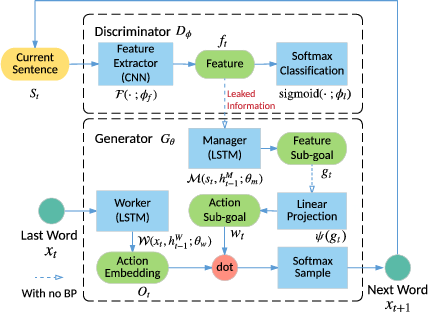
\includegraphics[width=.8\textwidth]{leakgan.png}
  \caption{Architettura di una LeakGAN \cite{LeakGAN}}
  \label{fig:leakgan}
\end{figure}

Queste reti vengono presentate in \cite{LeakGAN} e si differenziano dalle precedenti per due motivi:
\begin{itemize}
  \item si introduce una ``perdita'' (\emph{leak}) di informazione dal discriminatore al generatore.
    Le \emph{feature} che il primo estrae e su cui poi baserà la valutazione vengono fornite al secondo in modo da ricevere un'informazione molto più ricca di un semplice punteggio; 
  \item si introduce anche un nuovo modulo all'interno del generatore in modo da elaborare l'informazione che giunge da $D$ ed utilizzarla per poi decidere il token successivo.
\end{itemize}
Va subito fatto notare come la seconda modifica renda il generatore un generatore gerarchico, quindi composto da sottomoduli con specifici compiti.
È altrettanto importante sottolineare che i sotto-compiti che il Manager richiede al Worker sono auto-determinati, infatti i risultati ottenuti dimostrano che il Manger è in grado di richiedere al Worker la generazione di punteggiature e particolari strutture.

La \emph{Linear Projection} presente nello schema effettua una trasformazione lineare $\psi$, con pesi $W_\psi$, su un numero $c$ di goal $g_t$ recenti, così da generare un vettore $w_t$ di dimensione adeguata per l'esecuzione del prodotto con $O_t$.

\noindent
In formule si ha
\begin{align}
  w_t &= \psi \left( \sum_{i=1}^{c} g_{t-1} \right)
  \\
  O_t, h_t &= Worker(x_t, h_{t-1}; \theta)
  \\
  x_{t+1} = G_\theta(\cdot|s_t) &= softmax ( O_t \cdot w_t / \alpha)
\end{align}
in cui $h_t$ è \emph{hidden state} del Worker, mentre $\alpha$ viene usato per bilanciare esplorazione e sfruttamento (\emph{exploration and exploitation}).
In generale avrà un valore alto durante il \emph{training} per favorire l'esplorazione, avrà invece un valore basso durante la generazione di quelle sequenze che poi verranno usate per allenare $D$.

%\todo{spiegare meglio train G? Rescaled $R_t$?}

Un'altra importante modifica riguarda l'\emph{interleaved training}: si alternano allenamento tramite GAN ed allenamento tramite metodo supervisionato (MLE), anziché effettuare soltanto GAN dopo il \emph{pre-train}.
Questo evita il \emph{mode collapse} obbligando $G$ a rimanere aderente alla vera distribuzione degli esempi reali, evitando quindi che si specializzi su casi particolari con cui confondere $D$.
La modifica viene mostrata in modo esplicito a riga 4 del pseudocodice \textbf{Algorithm \ref{alg:LeakGAN}}.
Notare come vengano mostrati esplicitamente i parametri del Worker e del Manager, specificando che vengono aggiornati indipendentemente.

I risultati riportati in \cite{LeakGAN} mostrano come le LeakGAN siano in grado di superare le già buone prestazioni delle SeqGAN su sequenze di 20 token e come le superino notevolmente con sequenze lunghe 40 token.
Interessante anche il grafico ottenuto tramite PCA che permette di ottenere una visualizzazione della capacità delle LeakGAN di raggiungere lo spazio delle feature dei dati reali.

In \autoref{tab:esempi} vengono esposti quattro esempi generati da LeakGAN e SeqGAN allenate con le didascalie del dataset COCO.
\clearpage

\begin{algorithm}
  \caption{Adversarial Training with Leaked Information}
  \label{alg:LeakGAN}
  \begin{algorithmic}[1]
    \State Initialize $G_{\theta_m, \theta_w}$, $D_\phi$ with random weights $\theta_m$,$\theta_w$, $\phi$
    \State Pre-train $D_\phi$ on real data and generated data
    \State Pre-train $G_{\theta_m, \theta_w}$ using leaked information from $D_\phi$
    \State Perform the two parts of pre-training interleavingly until convergence
    \Repeat
      \For{g-steps}
        \State Generate a sequence $Y_{1:T} = (y_1, \dots, y_T) \sim G_{\theta_m, \theta_w}$
        \For{$t$ in $1:T$}
          \State Store leaked information from $D_\phi$
          \State Get $Q(f_t, g_t)$ by Monte Carlo Search
          \State Get the computed direction $g_t$ from MANAGER
          \State Update WORKER parameters $\theta_w$, $\psi$, softmax
          \State Update MANAGER parameters $\theta_m$
        \EndFor
      \EndFor
      \For{d-steps}
        \State Use current $G_{\theta_m, \theta_w}$ to generate negative examples
        \State Train $D_\phi$ for $k$ epochs on generated examples and real data
      \EndFor
    \Until{LeakGAN converges}
  \end{algorithmic}
\end{algorithm}

\begin{table}[ht]
\centering
\begin{tabular}{|l|} 
\hline
LeakGAN  \\
\hline
(1) A man sitting in front of a microphone with his dog sitting oh his shoulder. \\
(2) A young man is holding a bottle of wine in his hand.  \\
\hline
SeqGAN \\
\hline
(1) A couple of kids in a bathroom that is in a bathroom. \\
(2) A bathroom with tiled walls ad shower on it. \\
\hline
\end{tabular}
\caption{Esempi generati da modelli alleanti con \emph{COCO Image Captions}}
\label{tab:esempi}
\end{table}




%% ================================ %
%%           Bibliografia           %
%% ================================ %
\cleardoublepage
\printbibliography



\end{document}
